\newpage
\section{Qualità di processo}

	Per garantire la qualità del prodotto finale è necessario garantire la qualità dei processi necessari al suo completamento. A questo scopo, si è deciso di adottare lo standard \textit{ISO/IEC 15504\ped{G}}, denominato \textit{SPICE\ped{G}}.
	Esso si fonda sul principio che ogni processo deve essere controllato costantemente, in modo tale da rilevare possibili errori o debolezze, e correggerli prima che essi si diffondano, provocando un aumento del carico di lavoro e dello spreco di risorse.
	\textit{SPICE\ped{G}} definisce sei livelli di maturità del processo:
	
	\begin{itemize}
		\item \textbf{Level 0 - Incomplete:} processo non ancora implementato o incapace di raggiungere i suoi obiettivi;
		\item \textbf{Level 1 - Performed:} processo messo in atto e capace di raggiungere i suoi obiettivi;
		\item \textbf{Level 2 - Managed:} processo eseguito sulla base di obiettivi ben definiti;
		\item \textbf{Level 3 - Established:} processo eseguito in base ai principi dell’ingegneria del software; 
		\item \textbf{Level 4 - Predictable:} processo attuato all’interno di limiti ben definiti;
		\item \textbf{Level 5 - Optimizing:} processo predicibile e capace di adattarsi per raggiungere obiettivi specifici e rilevanti;
	\end{itemize}
	
	Al fine di perseguire correttamente questo modello, è necessario adottare il principio \textit{PDCA\ped{G}}, il quale si compone delle seguenti quattro fasi:
	
	\begin{itemize}
		\item \textbf{Plan:} fase di pianificazione ed individuazione di obiettivi e processi necessari allo scopo di raggiungere i risultati attesi;
		\item \textbf{Do:} fase di attuazione delle attività pianificate nella precedente fase e raccolta di dati sulla qualità ottenuta;
		\item \textbf{Check:} fase di verifica dove vengono confrontati i dati in uscita dalla fase Do con quelli pianificati nella fase Plan;
		\item \textbf{Act:} fase in cui si determinano le cause delle differenze fra risultati ottenuti e risultati attesi, in modo da individuare le azioni correttive da effettuare per ottenere un miglioramento della qualità.
	\end{itemize}

	\begin{figure}[H]
		\centering
		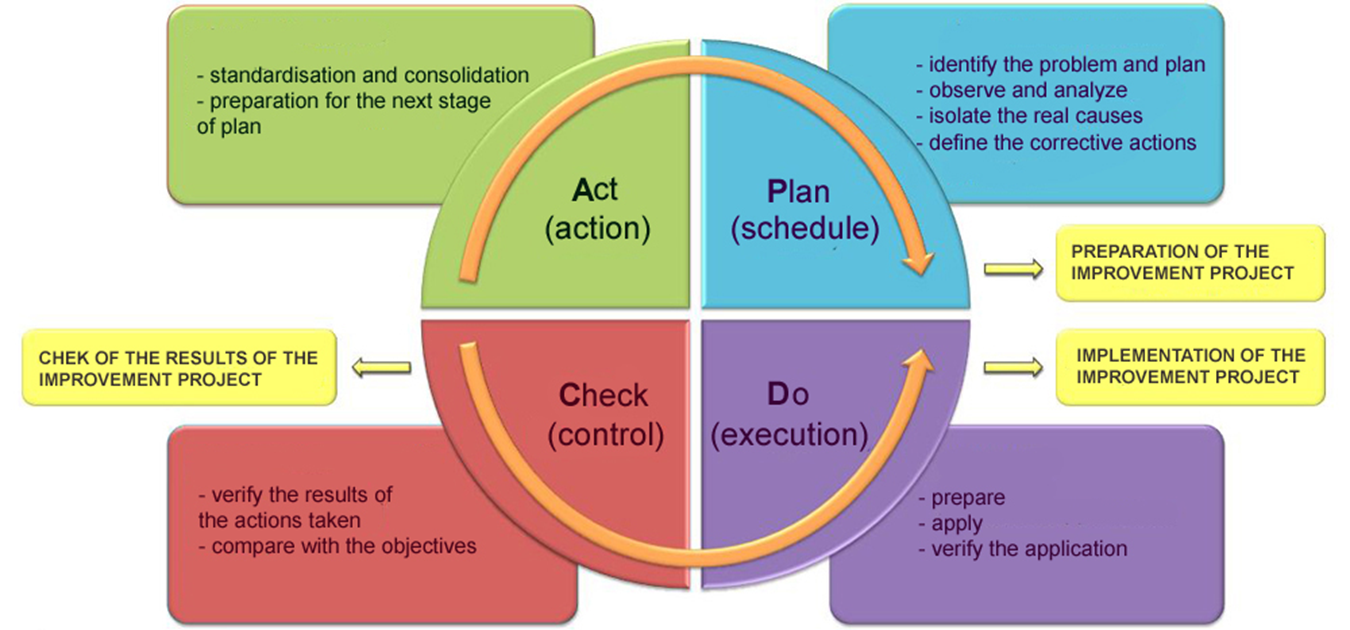
\includegraphics[scale=0.6]{includes/img/pdca.png}
		\caption{Fasi del principio PDCA.}
	\end{figure}

	Infine, il \textit{team\ped{G}} ha individuato dallo standard \textit{ISO/IEC 12207:2008\ped{G}} i processi che ritiene più importanti durante tutto il ciclo di vita del prodotto, al fine di garantire una buona qualità di processo. Per ognuno di essi sono stati individuati obiettivi e metriche coerenti con i livelli di qualità perseguiti.
	
	\subsection{Infrastructure Management Process (6.2.2)}
	
	\subsection{Project Planning, Assessment \& Control Process (6.3.1 - 6.3.2)}
	
	\subsection{Risk Management Process (6.3.4)}
	
	\subsection{System/Software Requirements Analysis Process (6.4.2 - 7.1.2)}
	
	\subsection{System/Software Architectural Design Process (6.4.3 - 7.1.3)}
	
	\subsection{Software Detailed Design Process (7.1.4)}
	
	\subsection{Software Construction Process (7.1.5)}
	
	\subsection{System/Software Integration Process (6.4.5 - 7.1.6)}
	
	\subsection{System/Software Qualification Testing Process (6.4.6 - 7.1.7)}
	
	\subsection{Software Documentation Management Process (7.2.1)}
	
	\subsection{Software Verification Process (7.2.4)}
	